\subsection{Theoretical framework: a normative principle linking variability, efficiency, and sparseness}

We define coding efficiency as $\mathrm{ICE} = I(s;r)/C$ and adopt the deterministic-encoding approximation ($H(r|s)\approx 0$, hence $I(s;r)\approx H(r)$), which holds when between-stimulus variability dominates trial-to-trial noise and provides an upper bound on achievable ICE when noise entropy is non-negligible.  For spontaneous activity, where no stimulus is defined, $H(r)$ is used directly as a measure of \emph{coding readiness}---the maximum information the network could transmit given its current metabolic state---rather than as an approximation to $I$ (Fig.~\ref{fig:figure1_conceptual_framework}A).  The optimization problem is
\begin{align}
\max_{p(r)} H(r)
\quad \text{s.t.}\quad
\mathbb{E}[c(r)] \le C,\;\; r\!\in[0,r_{\max}].
\label{eq:normative}
\end{align}

The unique solution has the Gibbs form
\begin{align}
p^*(r;C) = Z^{-1}(\beta)\,\exp[-\beta\,c(r)],
\label{eq:gibbs}
\end{align}
where the Lagrange multiplier $\beta = dH/dC$ is the \emph{marginal efficiency}---the incremental information gain per unit metabolic cost.  For linear cost $c(r)=r$, the optimal distribution is exponential with $\beta = 1/C$ and $H = \ln C + 1$ (Fig.~\ref{fig:figure1_conceptual_framework}B).

The family $\{p^{\star}(\cdot;\beta):\beta>0\}$ of optimal distributions forms the one-dimensional \textbf{Gibbs manifold (GM)} $H^\star(C)=\max_{p}\{H(p):\mathbb{E}_p[c]\le C\}$, the upper envelope of attainable $(C,H)$ in the entropy--cost plane (Fig.~\ref{fig:figure1_conceptual_framework}C\textit{i}).  Two derived quantities are defined along the manifold: the \emph{average efficiency} $\mathrm{ICE}(C)=H^\star(C)/C$ and the \emph{marginal efficiency} $\beta(C)=dH^\star/dC$; we plot these as the average-efficiency and marginal-efficiency curves, respectively, when needed.

Canonical firing statistics occupy different points: linear cost gives exponential ($\mathrm{CV}=1$, Poisson-like cortical firing \cite{4,5}), quadratic cost Gaussian-like, bounded cost approximately uniform; all three follow the same monotonic variability--cost structure (Supp.~Sect.~1).

The coefficient of variation $\mathrm{CV}=\sigma/\mu$ of $p(r)$ is an experimentally accessible coordinate along the manifold.  Three symbols throughout: plain $\mathrm{CV}$ for the theoretical (distributional) coordinate that the framework constrains; $\mathrm{CV}_P$ for the empirical population CV (across neurons, within a trial); $\mathrm{CV}_L$ for the empirical lifetime CV (across trials, per neuron).  $\mathrm{CV}_P, \mathrm{CV}_L$ are proxies bounded by biophysical constraints (refractory period, membrane time constant), so they may saturate while distributional $\mathrm{CV}$ continues to rise---we encounter this in Section~\ref{sec:single_neuron_ice}.  Each figure reports the CV variant it uses.

The CV behaviour along the manifold depends on the cost function.  Under unbounded linear cost $c(r)\propto r$ on $[0,\infty)$ the Gibbs solution is scale-invariant ($\mathrm{CV}\equiv 1$ for any budget).  Under bounded linear cost on $[0,r_{\max}]$ the truncated exponential yields $\mathrm{CV}\in[1/\sqrt{3},1]$, increasing monotonically with $\beta$ as the distribution concentrates near zero while preserving a heavy tail (Fig.~\ref{fig:figure1_conceptual_framework}C,i)---so increasing metabolic pressure drives activity toward simultaneously higher sparsity and higher variability.  Empirical CV values exceeding 1 (Figs.~\ref{fig:V1},~\ref{fig:network}) are accommodated by an effective phenomenological extension to sublinear cost $c(r)\propto r^\alpha$, $\alpha<1$, that produces heavier-tailed Gibbs distributions and admits a closed-form inversion CV$\to\hat\alpha$ (Supplementary Note ``Sublinear cost extension'').  This extension lies outside the convex-cost premise of the ICE--CV monotonicity theorem (Supp.~Sect.~1.4) and is presented as a fit rather than a strict prediction; numerical scans confirm that the ordering is preserved over the relevant $\alpha$ range.

Along the manifold, three properties of distinct logical status emerge (Fig.~\ref{fig:figure1_conceptual_framework}C):
\begin{itemize}
    \item \emph{Sparseness--variability coupling.} An algebraic identity: the moment-based Treves--Rolls sparseness satisfies $S = \mathrm{CV}^2/(1+\mathrm{CV}^2)$ in the large-$N$ limit, so $S$ and CV are coupled whenever they are computed over the same non-negative response samples (panel~ii).  The relation is independent of the Gibbs optimization and does not extend automatically to ISI-based CV, Fano factor, or noise correlations.

    \item \emph{Efficiency--variability coupling.} A normative prediction under the Gibbs structure: within the strictly-convex-cost regime, both $\beta$ and $\mathrm{ICE}=H/C$ increase with CV along the optimal family, following from the strict concavity of $H^\star(C)$, $\mathrm{Var}(c)>0$, and the non-negative-entropy convention $H^\star(0)\ge 0$ that holds automatically for discrete spike-count entropies (Supp.~Sect.~1.5; panel~iii).  In the sublinear-cost extension used for CV$>1$ data the convexity premise is violated and monotonicity is supported by numerical scans only.  The same monotonic ordering holds for Poisson, Gaussian, and Uniform families under matched parameter sweeps (Supp.~Sect.~2.2), a distributional robustness check along specific parameter paths.

    \item \emph{Spike-count-agreement--variability coupling.} A model-dependent implication under Poisson statistics: $P_{\mathrm{agree}}(\lambda)=e^{-2\lambda}I_0(2\lambda)$ with $\lambda=\mathrm{CV}^{-2}$ rises monotonically with CV (Supp.~Sect.~2.3; panel~iv).  We treat this as a restricted form of reliability and not as decoder-based stimulus discriminability; for fixed-$\sigma$ families (Gaussian, Uniform) the same metric is CV-invariant.
\end{itemize}

In the experimental sections below, information and cost are instantiated differently per context (see Methods); units are not comparable across contexts and the empirical claim is the within-pairing monotonic ICE--CV relationship rather than an absolute collapse.  The per-context bookkeeping ($H/C$ vs.\ $I/C$, evoked vs.\ spontaneous interpretation, role of each quantity) is tabulated in Supplementary Table~S5.

\begin{figure*} [t!]
\centering 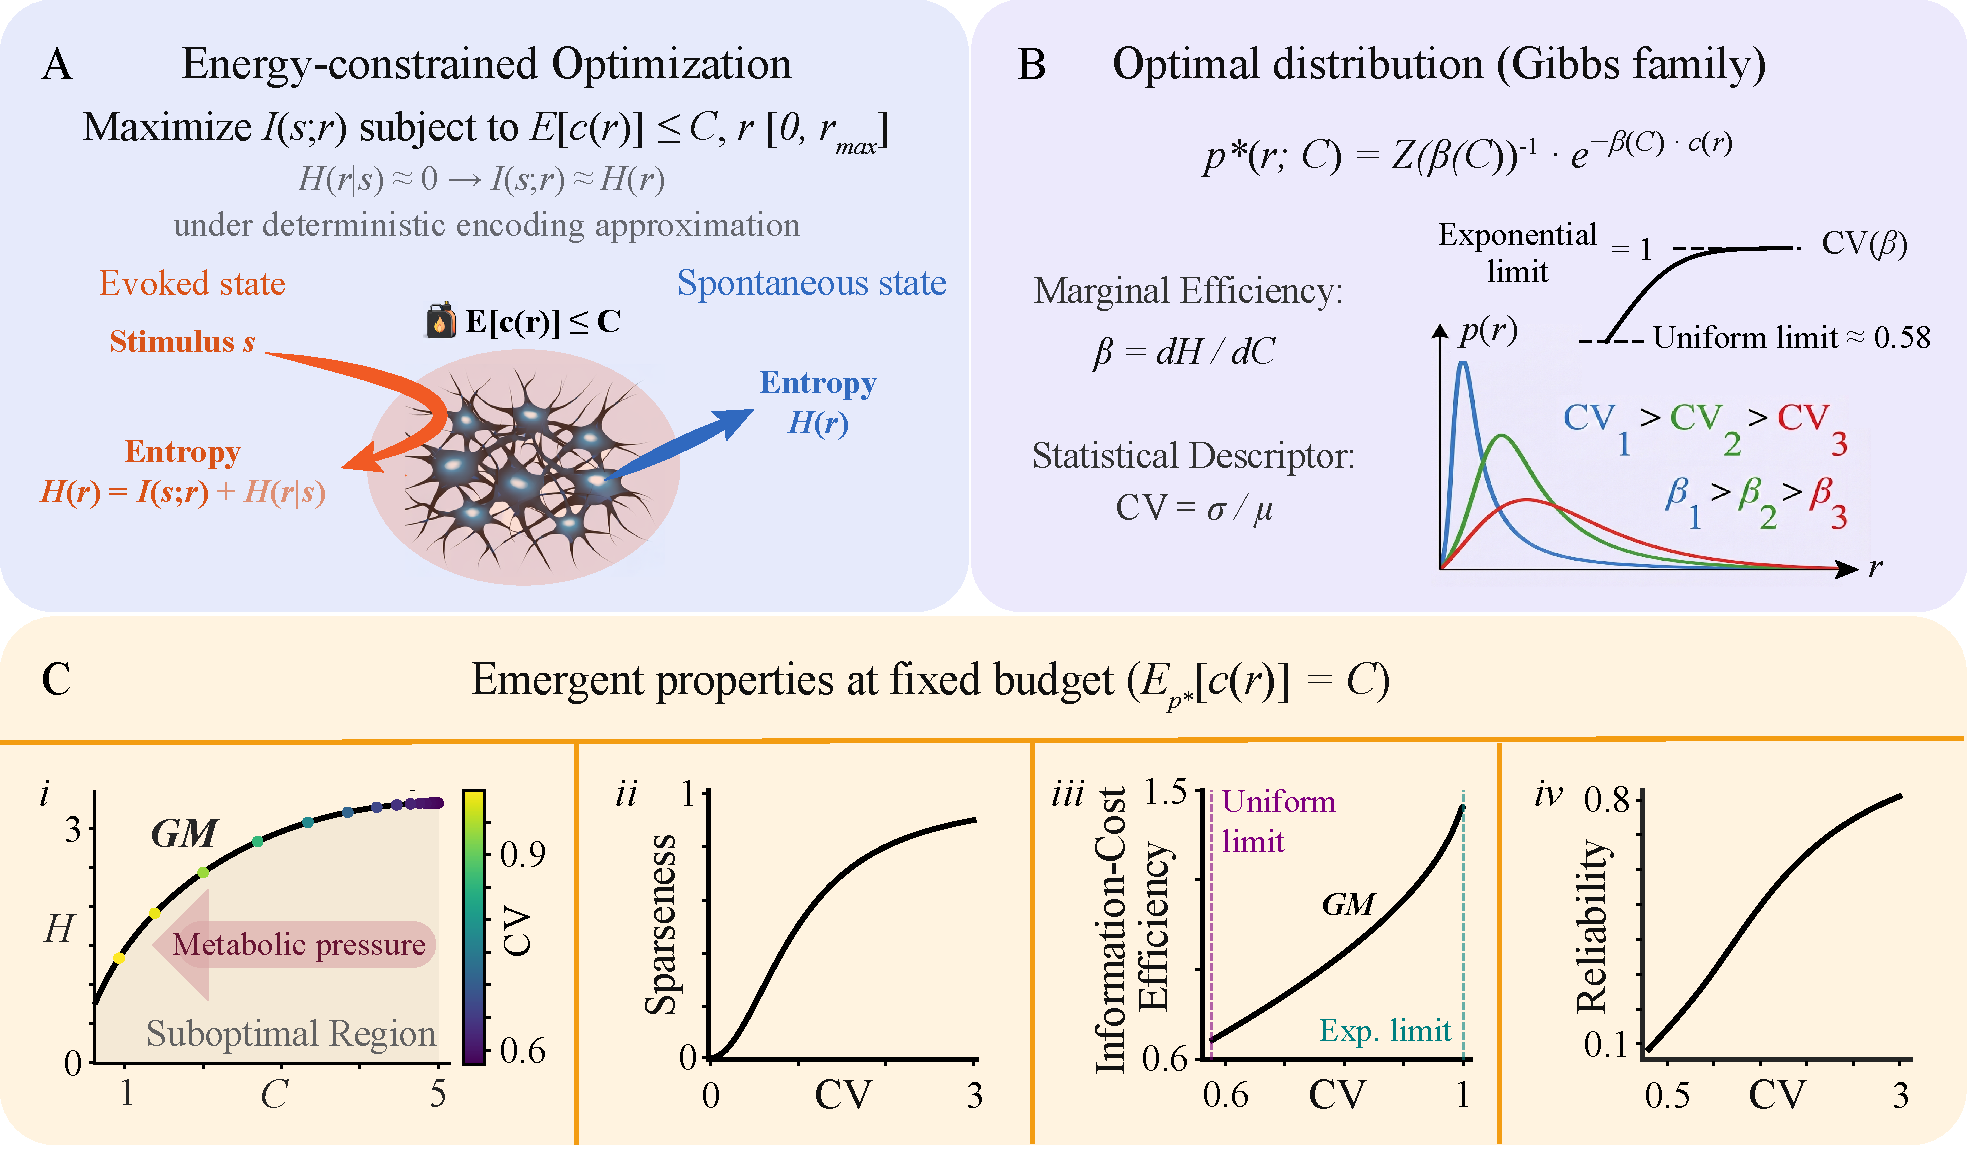
\includegraphics[scale=0.39]{figures/Figure1.pdf}
\caption{\textbf{Conceptual framework for energy-constrained efficient coding.}
(\textbf{A}) \textbf{Energy-constrained optimization.}  Maximize $I(s;r)$ subject to $\mathbb{E}[c(r)]\le C$ on $r\in[0,r_{\max}]$.  Under the deterministic-encoding approximation $H(r|s)\approx 0$, $I(s;r)\approx H(r)$, so the problem reduces to entropy maximization under the budget.  Evoked (orange): $H(r)=I(s;r)+H(r|s)$.  Spontaneous (blue): no stimulus is defined; $H(r)$ is read as \emph{coding readiness}, not as an approximation to $I$.
(\textbf{B}) \textbf{Optimal distribution (Gibbs family).}  $p^*(r;C) = Z(\beta(C))^{-1}\,e^{-\beta(C)\,c(r)}$, with marginal efficiency $\beta=dH/dC$ and descriptor $\mathrm{CV}=\sigma/\mu$.  Three example densities (blue/green/red): $\beta_1>\beta_2>\beta_3$ (tight $\to$ loose budget) with correspondingly higher CV.  Inset $\mathrm{CV}(\beta)$ runs between bounded-cost limits: uniform ($\mathrm{CV}\approx 0.58$, $\beta\to 0$) and exponential ($\mathrm{CV}=1$, $\beta\to\infty$).  Under unbounded linear cost the solution is scale-invariant and $\mathrm{CV}\equiv 1$; the $\beta$--CV coupling requires bounded $r$ or nonlinear cost.
(\textbf{C}) \textbf{Emergent properties at fixed budget} ($\mathbb{E}_{p^*}[c(r)]=C$).  (\textbf{i}) Gibbs manifold (GM) $H^\star(C)$ in the entropy--cost plane above the suboptimal region; CV (colorbar) rises along the manifold as the budget tightens (arrow).  (\textbf{ii}) Sparseness vs.\ CV (\emph{algebraic identity}, saturates at 1).  (\textbf{iii}) ICE vs.\ CV (\emph{Gibbs prediction}); under bounded linear cost the curve runs between the uniform and exponential limits.  (\textbf{iv}) Trial-to-trial spike-count agreement $P_{\mathrm{agree}}$ vs.\ CV (\emph{Poisson-regime corollary}; CV-invariant for fixed-$\sigma$ Gaussian/Uniform; the panel-iv label ``Reliability'' is shorthand for this restricted count-agreement metric).  At very low rates the rise is partly silence-induced; an FR-controlled V1 decoder analysis tests the link beyond the Poisson algebra (Section~\ref{sec:network_results}).}
\label{fig:figure1_conceptual_framework}
\end{figure*}

